
Information is incredibly important in programming,
whether it is what a command does, how its used,
or what is contained in variables.
I take information as a starting point,
and this section is all about obtaining and storing various forms of information.


\subsection{The \texttt{help} command}\label{sec:hlp}

Perhaps the most important command in Stata,
\texttt{help} allows quick access to information on \emph{any} command Stata has.
The help-files Stata provides are incredibly detailed,
including information on how to use the command (its \emph{syntax}),
what the command does, its output, examples,
and sometimes even the theory behind it.
As useful as it is, the help-files might seem daunting at first.
Understanding their structure is key to (quickly) obtain information without falling into despair.
I'll highlight what I believe to be the most important parts of the help-files through an example.

If I type \st{help summarize},
Stata opens the window in \cref{fig:hlpsum}.
In help-files, the typography on its own already gives us a lot of information.

\textbf{Bold} words indicate commands or options; if we want to use these,
we type them exactly as they are written down.
In our case,
\textbf{\texttt{summarize}} is written in bold under the syntax heading.
It is, as we know, indeed a command.

\textit{Italicised} text indicates something that should be substituted.
Here, \textit{\texttt{varlist}} tells us that we should write down a list of variable names here -- should we want to use this option.

Optional arguments and functions are indicated by being [in brackets].
This means that anything that is written within brackets in the syntax is something that does not have to be specified for a command to work.

\underline{Underlined} text indicates the \emph{minimum} abbreviation of a command or option.
In the case of \st{summarize},
I could simply write \st{su}.
Additional letters are also allowed and how to use this is mostly personal preference.
Personally, I always write \st{sum} as it's clearer to me what that means than \st{su},
but it still saves me the time and space from writing the command out in its entirety.
When abbreviating commands,
make sure you are familiar enough with them to remember what an abbreviation means if you open your do-files one week later.\footnote{%
To get you used to abbreviated commands,
I'll abbreviate most commands as I would do when using them in my own code after I have introduced them.
The other reason is that I'm lazy and don't like typing.}
Having to look it up every time you see an abbreviation can be quite a pain.

Finally, any text in \textcolor{blue}{blue} is a hyperlink,
generally leading to more information on whatever is written down.\footnote{Note that the exact colour depends on Stata's colour scheme, but the default and dark schemes do use blue.}

\begin{figure}[tbp]\centering
  \caption{Help-file for \texttt{summarize}}\label{fig:hlpsum}
  \vspace{1ex}
  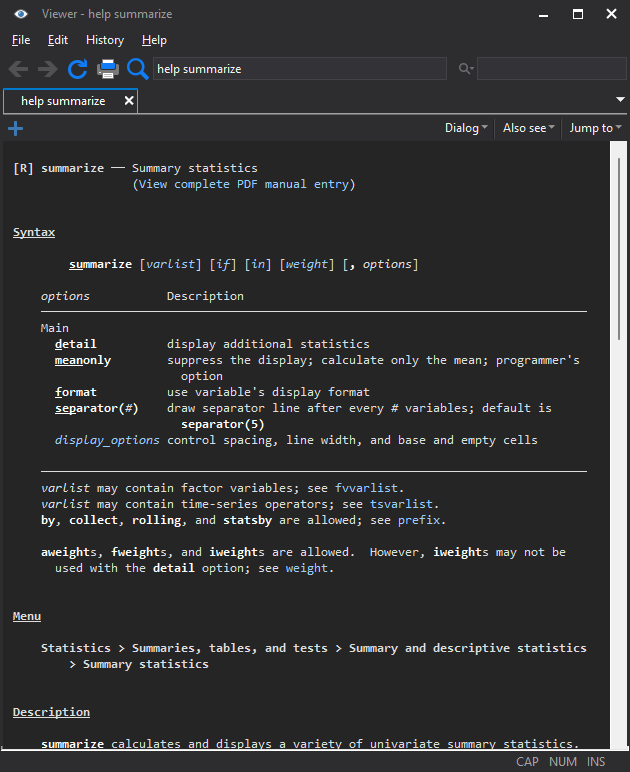
\includegraphics[width=0.85\textwidth]{helpsummarize}
\end{figure}

\subsection{Storing Information}

\subsubsection{Scalars and matrices}

Rather than storing information in variables,
Stata offers us a couple of different ways of storing information independently of a datset.
Scalars and matrices are perhaps the most basic of these options.
Other than the names suggest, scalars are not limited to containing only numbers:
we are free to store other types of information such as strings in them as well.
Matrices can only contain numerical values, on the other hand.
Another difference between the two is the amount of information stored:
a scalar contains a single piece of information,
whereas a matrix can contain multiple pieces of information.

Scalars can be created using the \st{scalar define} command,
although the \st{define} can be left out.
For example,
if I want to create a scalar containing the number 7,
I could type:
\begin{minted}{stata}
  scalar define number = 7
\end{minted}
but also:
\begin{minted}{stata}
    scalar number = 7
\end{minted}

After running this line of code -- either through a do-file or the Stata console -- Stata has now created a scalar with the name ``number'' that contains the numerical value 7.
Naturally, we cannot always remember every piece of information we have stored.
If we want to know what scalars currently exist in Stata's memory, we use another command:
\begin{minted}{stata}
  sca def number = 7
  sca second = "two"
  sca list
\end{minted}
After running the second command, Stata returns us a list of all scalars with both their name and value:
\small\begin{verbatim}
  . sca list
      second = two
      number =          7
\end{verbatim}\normalsize
Note that we can also type \st{dir} instead of \st{list} and obtain the same result.

Compared to scalars, matrices are both more versatile and more complicated to work with.
As they store multiple pieces of information, every piece of information also needs a position.
Creating a matrix is slightly different compared to creating a scalar:
\begin{minted}{stata}
  matrix input numbers = ( 7 , 2 \ 1 , 2)
\end{minted}
This creates a two by two matrix (i.e.\ two rows and two columns),
containing the values 7 and 2 in the first row and the values 1 and 2 in the second row.
In this command, commas seperate row values while backslashes start a new row.
Again, \st{input} can be omitted when creating a matrix.
There is also a \st{matrix define} command,
but this is used when we do computations with already existing matrices.
\st{input} is used when inputting matrices by hand.

To see existing matrices, we use two commands:
\begin{minted}{stata}
  matrix input numbers = ( 7 , 2 \ 1 , 2)
  mat dir
  mat list numbers
\end{minted}
The first of these shows us a list of all matrices in Stata's memory and their size,
while the second command shows us the values of the matrix called ``numbers'':
\small\begin{verbatim}
  .   mat dir
        numbers[2,2]

  .   mat list numbers

  numbers[2,2]
      c1  c2
  r1   7   2
  r2   1   2
\end{verbatim}\normalsize

Finally,
we can remove scalars and matrices from Stata's memory using their respective command followed by \st{drop}:
\begin{minted}{stata}
sca drop _all
mat drop numbers
\end{minted}
We can remove a specific scalar or matrix by specifying its name,
or we can remove all existing scalars or matrices by typing \st{_all} instead of a name.
Scalars and matrices are also removed from memory when you close Stata itself or when you issue the \st{clear all} command.

The \st{help} file for both commands provide a lot more information on both scalars and matrices, especially so for the latter.
Also note that, especially for matrices, a lot is possible using Stata's underlying programming language Mata.
Unless you plan on writing elaborate and complex estimation commands,
you will likely never need or encounter Mata;
it is thus beyond the scope of this reader -- for now.\footnote{At the moment, I do not have a lot experience with Mata yet, either. Although writing a guide on it would likely be a quick way for me to learn it, I do not think it would add much value for this reader. I might change my mind about this later, though.}

\subsubsection{Macros}

Stata recognises two types of macros: \st{global}s and \st{local}s.
If you are not familiar with the term,
a macro is basically a shorthand or abbreviation:
instead of repeatedly typing out some very long string of characters,
we can define and use a macro instead, saving space, time,
and keeping our code much more organised.

\paragraph{Locals}
Of the two macro types, the local is most common.
The major (dis)advantage of a local is that Stata ``forgets'' it after running the code it is defined in.
This means we cannot use locals interactively:
if we define a local in Stata's command line,
it will be gone by the time we execute a second command.
At the same time,
this also means we can repeatedly redefine the contents of a local without having to drop it after every time we run a block of code,
and, more importantly, locals in our programs won't interfere with locals of other programs.

The basic syntax for defining a local is relatively simple:
\begin{minted}{stata}
local name contents
\end{minted}
All we need is to indicate that we are defining a \st{local}, give it a name,
and provide its content.
To use the local, we need to tell Stata to expand it in our following command(s).
We do this by surrounding the local's name by a single opening and closing quote, i.e. \st{`name'}.
Note that you \emph{have} to use the separate opening and closing quote characters,
using a single closing quote twice --
as you would in a regular text processor such as Word\footnote{%
Most modern text processors automatically change the straight quotes of our keyboard into opening or closing quotes,
depending on the surrounding characters.
Most programming environments don't:
you generally aren't writing text in a programming environment, but code.} --
will generally cause Stata to return an error,
as it does not recognise our local as such.
In short: write \st{`name'}, not \st{'name'}.

To make the concept a little less abstract, I'll provide an example.
Suppose you have a large amount of regressions or other estimation commands you want to run,
all with the same control variables.
Instead of typing out all the variable names every time,
we can define a local with the variable names and use that instead.
\cref{lst:local} does just this, and you can copy the code into a do-file and try for yourself.

\begin{listing}[tbp]
\caption{local.do}\label{lst:local}
\inputst{local.do}
\end{listing}

\paragraph{Globals}
Where a local is a \emph{private} macro available only to the code it is defined in,
a global is a \emph{public} macro and is available to other programs or code as well.
While this can be very helpful for anything used often in more than just a single do-file or program, this comes with a caveat.
Every global name is available only once,
i.e. if one program defines a global named ``myglobal'',
any other program attempting to define a global with this name will overwrite the previous contents of ``myglobal''.
This can therefore interfere when running code written by others:
if their code uses or defines a global with the same name as one of your globals,
either their code or yours will likely not work as intended.
It is thus best practice to avoid using globals wherever possible,
e.g. by using locals instead.

Nevertheless, globals do have their uses.
An example would be to define the path to the folder in your current project,
so you can use the global instead of typing out the entire path every time you would refer to some file.\footnote{%
While this helps in making sure your code always uses the correct files,
you can also open Stata from the project folder and refer directly to file names.
The downside of the latter method is that you always need to make sure Stata has the correct working directory when executing your code.
You can check and change the current working directory with the commands \st{pwd} and \st{cd}, respectively.}

The syntax for globals is slightly different compared to locals, but they are otherwise handled in the same manner.
To define a global, we type \st{global name contents} and we can expand a global by affixing a dollar sign before its name, like so: \st{$name}. $\) % added inline math to stop syntax highlighting

\paragraph{General remarks and usage tips}
Before moving on, I'd like to highlight several other ways to manipulate or define macros.
Instead of simply storing information we spell out,
a macro can also be defined through an \emph{expression} or through a \emph{macro function}.
To put it simply,
using an expression tells Stata to evaluate the expression and store the result,
while a macro function tells Stata to obtain the information defined through the function.
The syntax for using an expression is \st{local name =expression},
and the syntax for using a macro function is \st{local name : function}.

To illustrate the use of an expression, consider the following code:
\begin{minted}{stata}
loc sum 1 + 1
loc sum2 = 1 + 1
\end{minted}
When we evaluate these, the first (\st{`sum'}) will expand to \st{1 + 1},
while the second (\st{`sum2'}) will expand to \st{2}.
By using an expression,
we basically told Stata to calculate 1 + 1 and store the result of that.
The reason Stata does not evaluate the contents in the first local is that unless specified otherwise,
Stata implicitly places double quotes surrounding the contents.
In other words, writing \st{local name contents} is exactly the same as writing \st{local name "contents"}.
Of course, there are cases where we would want to manually add quotes,
but I'll get into the details of using double quotes in Stata programming later.
For a list of available macro functions, see \st{help macro#macro_fcn}.

After defining a macro, we can manipulate it in the same manner as defining it.
To do this, we simply define the macro again: \st{local name contents}.
This will simply throw away the previous contents and store whatever new contents you define.
If we want to keep the previous contents,
we can expand the current local inside its new contents:
\st{local name `name' newcontents} or \st{local name newcontents `name'}.
This would add new content to the local after or before the current contents,
respectively.

We can also use locals as a sort of counter.
If we define a local as an integer,
we can use a shorthand for incrementing the local.
For example:
\begin{minted}{stata}
loc counter 1
loc counter = `counter' + 1
loc ++counter
loc counter++
\end{minted}
After defining the local in the first line,
lines 2--4 all increment the local by one,
so that the local expands to 4 if it is used afterward.
This is mainly useful when using a local inside loops,
which we will get into later in this reader.

In general, macros are extremely flexible,
especially if we combine the several ways of manipulating them.
I wholeheartedly recommend practicing a bit in using them,
as they can save an enormous amount of time spent coding --
both by reducing the amount you need to type out and by making your code much more readable.

\subsection{Inspecting and Obtaining Information}
Now that we now how to store information,
we also need to consider how to obtain information or inspect what information has been stored.
I've already covered how to find information on commands (\cref{sec:hlp}),
and you've likely inspected a dataset before using the \st{describe} or \st{browse} commands.
These are all very helpful, but it is now time to delve into handling nitty-gritty specific pieces of information.

\subsubsection{The \texttt{display} command}
The \st{display} command is one of -- if not the -- most used commands for me while programming.
It's function is quite simple: it displays whatever you tell it to in Stata's output window.
Furthermore, it evaluates whatever you tell it to display (unless specified otherwise),
so you can also use it as a calculator if you so desire.
The basic syntax is as follows: \st{display contents}.
If we insert any sort of calculation, display gives us the results:
\st{di 1 + 1} returns \st{2}.
If we do not want the contents to be evaluated, we enclose them with double quotes.
As an example,
let's define a local containing an expression and display it with and without double quotes.
Code for this is in \cref{lst:dsp}.

\begin{listing}[tbp]
\caption{display.do}\label{lst:dsp}
\inputst{display.do}
\end{listing}

If you execute this code, you'll see that the command in line 5 returns \st{6},
while the command in line 8 returns the expression as we wrote it:
\st{(1 + 1) * 3}.
The latter is especially useful if we automate the manipulation of locals and want to see if the contents are as expected.
Note also that if we want to display a string of text we \emph{need} to enclose it with double quotes as well,
otherwise Stata will interpret it as the name of a stored object,
such as a variable or scalar.

\paragraph{Quotes}
The more we start automating things,
the likelier it will be that one of the strings we store will itself contain quotes.
As both the starting and the ending symbol of quotes are similar,
this can quickly produce unintended results.
Suppose we create a local with such a string and tell Stata to display it:
\begin{minted}{stata}
// define local
loc quote Using quotes without thinking is a "wonderful" idea.

// display the local
di "`quote'"
\end{minted}
If we run this code, Stata returns an error.
To see where this goes wrong,
we can manually ``expand'' the local and see what we \emph{actually} told Stata to do:
\begin{minted}{stata}
    di "Using quotes without thinking is a "wonderful" idea."
\end{minted}
The problem here is that we did not provide a single string of text,
but two, with some word, \st{wonderful}, in between.
Stata does not recognise what ``wonderful'' means and thus doesn't know what to do.
The issues is that Stata does not know the order or hierarchy of the double quotes we've written: they're all the same character.
Luckily, there's a fix for this: \emph{compound} double quotes.
Instead of just writing ``normal'' double quotes,
we indicate whether it is a starting or an ending double quote.
To do this, we add a single opening or closing quote -- the same characters used for local expansion.
Let's build on the previous example and add the ``correct'' command in \cref{lst:quote} to illustrate.
To make sure the code runs,
I've commented out the incorrect command.

\begin{listing}[tbp]
    \caption{quote.do}\label{lst:quote}
    \inputst{quote.do}
\end{listing}

As your code (and locals) become more complicated,
all these different kinds of quotes can quickly make it difficult to see where everything starts and ends.
It took me ages to completely understand how and when to use these compound double quotes,
so don't worry if looks like abracadabra -- it often still does to me.
Practice makes perfect.

\paragraph{Display options}
The \st{display} command also has options to format the output.
While they don't make much of a difference for things like troubleshooting,
they can be nice if you're writing an extensive program and want to differentiate between specific types of output.
The options and an example of their use are provided in the official help file: \st{help display}.

\subsubsection{Results of other commands}
While working with Stata,
you probably don't want to write every bit of code from scratch:
there are already tons of useful commands available -- shipped with Stata or written by other users, so why not build on those?
Luckily,
Stata stores lots of information obtained and produced by any well-written command.
In general, (almost) all Stata commands are either \emph{r-class} or \emph{e-class},
corresponding to general commands and estimation commands, respectively.
General commands store their results in \st{r()} objects,
while estimation commands store their results in \st{e()} objects.
To access these results, we need to know the name of the object they are stored in.
Of course, there is a command to find out the names of the available objects.
For general commands we use \st{return list}, while we use \st{ereturn list} for estimation commands.
There is also a \emph{c-class} with \st{c()} objects,
but they are not related to commands and always available.
We can use \st{creturn list} for these.
\cref{lst:return} provides an example how to use this.

\begin{listing}[tbp]
    \caption{return.do}\label{lst:return}
    \inputst{return.do}
\end{listing}

Note that we do not have to use the various return commands every time we want to access one their corresponding objects;
they simply list what is available.
In a similar manner to how I display the contents of the objects in \cref{lst:return},
we can also store them in locals or use them in pretty much any other way you can think of.
